\chapter{Seamless Shift of Focus} \label{chapter4}
\minitoc
\eject

The evolution of the economical constraints of a web application requires to continuously shift from productivity to efficiency.
The incompatibility of platforms between the two organizations implies technological ruptures during this evolution.
Huge developing efforts are pulled to translate manually from one organization into the other, and later to maintain the implementation despites its unmaintainable nature.

In this chapter, section \ref{chapter4:equivalence} introduces the solution developed in this thesis.
A platform allowing to follow the development of a web application with a seamless shift of focus, from the productivity required in the early beginning until the efficiency required during maturation.
It is based on the transformation of an event-driven program to target a pipeline architecture.
Section \ref{chapter4:event-driven} presents the event-driven execution model on which relies the transformation.
And section \ref{chapter4:pipeline} presents the pipeline architecture targeted by the transformation.

\begin{figure}[h!] \label{fig:state-of-the-art-proposition}
\begin{center}
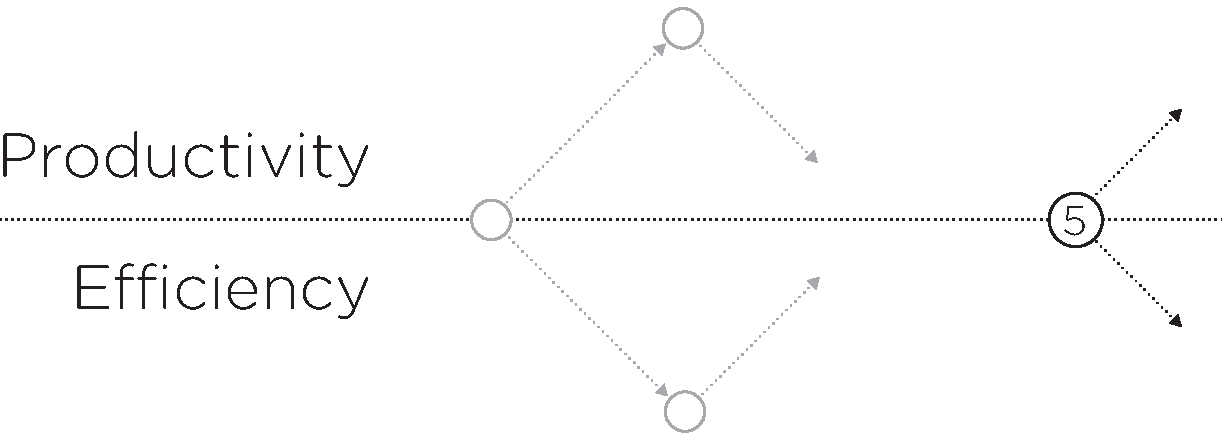
\includegraphics[width=0.6\textwidth]{../resources/state-of-the-art-5.pdf}
\end{center}
\end{figure}

\section{From Continuations to Dues} \label{chapter5:equivalence}

This section presents the transformation from a nested imbrication of continuations into a chain of Dues.
It explains the three limitations imposed by the compiler for this transformation to preserve the semantic.
They preserve the execution order, the execution linearity and the scopes of the variables used in the operations.

\subsection{Execution order}

The compiler spots function calls with a continuation, which are similar to the abstraction in (\ref{eq:order:source}).
It wraps the function $fn$ into the function $fn_\textbf{due}$ to return a Due.
And it relocates the continuation in a call to the method $\textbf{then}$, which references the Due previously returned.
The result should be similar to (\ref{eq:order:target}).
The differences are highlighted in bold font.
\begin{equation} \label{eq:order:source}
fn([arguments], continuation)
\end{equation}
\begin{equation} \label{eq:order:target}
fn_\textbf{due}([arguments])\textbf{.then}(continuation)
\end{equation}

The execution order is different whether $continuation$ is called synchronously, or asynchronously.
If $fn$ is synchronous, it calls the $continuation$ within its execution.
It might execute $statements$ after executing $continuation$, before returning.
If $fn$ is asynchronous, the continuation is called after the end of the current execution, after $fn$.
The transformation erases this difference in the execution order.
In both cases, the transformation relocates the execution of $continuation$ after the execution of $fn$.
For synchronous $fn$, the execution order changes ; the execution of $statements$ at the end of $fn$ and the continuation switch.
The latter must be asynchronous to preserve the execution order.

\subsection{Execution linearity}

The compiler transforms a nested imbrication of continuations, which is similar to the abstraction in (\ref{eq:state:source}) into a flatten chain of calls encapsulating them, like in (\ref{eq:state:target}).
\begin{align} \label{eq:state:source}
&fn1([arguments], cont1 \{\nonumber\\
&\qquad  declare ~ variable \leftarrow result\nonumber\\
&\qquad  fn2([arguments], cont2 \{\nonumber\\
&\qquad\qquad    print ~ variable\nonumber\\
&\qquad  \})\nonumber\\
&\})
\end{align}
\begin{align} \label{eq:state:target}
&\textbf{declare variable}\nonumber\\
&fn1_\textbf{due}([arguments])\nonumber\\
&\textbf{.then}(cont1\{\nonumber\\
&\qquad  variable \leftarrow result\nonumber\\
&\qquad  fn2_\textbf{due}([arguments])\nonumber\\
&\})\nonumber\\
&\textbf{.then}(cont2\{\nonumber\\
&\qquad  print ~ variable\nonumber\\
&\})
\end{align}

An imbrication of continuations must not contain any loop, nor function definition that is not a continuation.
Both modify the linearity of the execution flow which is required for the equivalence to keep the semantic.
A call nested inside a loop returns multiple Dues, while only one is returned to continue the chain.
A function definition breaks the execution linearity.
It prevents the nested call to return the Due expected to continue the chain.
% And a call nested inside a function definition is unable to return the Due to continue the chain.
On the other hand, conditional branching leaves the execution linearity and the semantic intact.
If the nested asynchronous function is not called, the execution of the chain stops as expected.

% We demonstrate the equivalence with a sequence of two continuations.
% The equivalence is sound for a sequence of \textit{n} continuations.

\subsection{Variable scope}

In (\ref{eq:state:source}), the definitions of $cont1$ and $cont2$ are
overlapping. The $variable$ declared in $cont1$ is accessible in $cont2$ to be
printed. In (\ref{eq:state:target}), however, definitions of $cont1$ and
$cont2$ are not overlapping, they are siblings. The $variable$ is not
accessible to $cont2$. It must be relocated in a parent function to be
accessible by both $cont1$ and $cont2$. To detect such variables, the compiler
must infer their scope statically. Languages with a lexical scope define the
scope of a variable statically. Most imperative languages present a lexical
scope, like C/C++, Python, Ruby or Java. The subset of Javascript excluding
the built-in functions \texttt{with} and \texttt{eval} is also lexically
scoped. To compile Javascript, the compiler must exclude programs using these
two statements.


\section{Event-Driven Execution Model} \label{chapter4:event-driven}

The event-driven execution model cooperatively schedules a queue of tasks to process events sequentially.
The developer defines the concurrent tasks as continuations.

\subsection{Continuation Passing Style} \label{chapter4:event-loop:continuation}

% A callback is a function passed as a parameter to a function call.
% It is invoked by the callee to continue the execution with data not available in the caller context.
% We distinguish three kinds of callbacks.

% \begin{description}
%   \item[Iterators] are functions called for each item in a set, often synchronously.
%   \item[Listeners] are functions called asynchronously for each event in a stream.
%   \item[Continuations] are functions called asynchronously once a result is available.
% \end{description}

% In a synchronous paradigm, the sequentiality of the execution flow is trivial.
% An operation needs to complete before executing the next one.
% In an asynchronous paradigm, parallelism is trivial, but the sequentiality of operations needs to be explicit.
In event-driven execution model, the scheduling between asynchronous, concurrent tasks is defined only by their causality.
They are not globally ordered.
% of the asynchronous execution flow
The causality between two tasks is defined using a continuation  \cite{Wand1980,Haynes1984}.
% A continuation is the functional way of defining the causality between two tasks \cite{Wand1980,Haynes1984}.
It is a function passed as an argument to a function call.
% The caller is able to continue the execution while the callee runs in background.
The continuation is invoked later, at the completion of the callee, to continue the execution. % as soon as possible and process the result; hence the name continuation.
It allows the callee not to block the caller until its completion.
% It provides a necessary control over the asynchronous execution flow.
% It also brings a control over the data flow which essentially replaces the \texttt{return} statement at the end of a synchronous function.
At its invocation, the continuation retrieves both the caller context, through a closure, and the result.
Listing \ref{lst:continuation} illustrates an example of continuation in \textit{Node.js}.

% The convention on how to hand back the result must be common for both the callee and the continuation.
% For example, in \textit{Node.js}, the signature of a continuation uses the \textit{error-first} convention.
% % \ftnt{https://docs.nodejitsu.com/articles/errors/what-are-the-error-conventions}
% % \ftnt{http://programmers.stackexchange.com/questions/144089/different-callbacks-for-error-or-error-as-first-argument} convention.
% The first argument contains an error or \texttt{null} if no error occurred; then follows the result.
% Listing \ref{lst:continuation} is a pattern of such a continuation.
% However, continuations don't impose any conventions; indeed, other conventions are used in the browser.

\begin{code}[js, %
             caption={Example of a continuation}, %
             label={lst:continuation}] %
my_fn(input, function continuation(error, result) {
  if (!error) {
    console.log(result);
  } else {
    throw error;
  }
});
\end{code}

% % The continuation allows to continue the execution sequentially, after the result of \textit{my_fn} is available. 
% % When continuations are defined inside the call, like \textit{continuation}, the sequence of deferred execution results in an intricate imbrication of calls and continuations, like in listing \ref{lst:cbhell}.
% The callback hell occurs when many asynchronous calls are arranged to be executed sequentially.
% Each consecutive operation adds an indentation level, because it is nested inside the continuation of the previous operation.
% % That is when each caller must wait for the result before calling the next function.
% It produces an imbrication of calls and function definitions, as shown in listing \ref{lst:cbhell}.

The continuation passing style lacks the chained composition of multiple asynchronous operations.
It forces to stack calls of continuations, as illustrated in listing \ref{lst:cbhell}.
Promises allow to arrange such a sequence of asynchronous operations in a chain, similar to a pipeline.


\begin{code}[js, %
             caption={Example of a sequence of continuations}, %
             label={lst:cbhell}] %
my_fn_1(input, function cont(error, result) {
  if (!error) {
    my_fn_2(result, function cont(error, result) {
      if (!error) {
        my_fn_3(result, function cont(error, result) {
          if (!error) {
            console.log(result);
          } else {
            throw error;
          }
        });
      } else {
        throw error;
      }
    });
  } else {
    throw error;
  }
});
\end{code}

\subsection{Promise} \label{chapter4:event-loop:promise}

% TODO insert these :
% Promise also provide few methods to enhance the asynchronous control flow tools\footnote{\texttt{all} and \texttt{race}}.
% There is, in Javascript, numerous Promise implementations\footnote{37 different implementations in Javascript \url{https://github.com/promises-aplus/promises-spec/blob/master/implementations.md}}.

% This section is based on the Promises section of the specification in ECMAScript 6 Harmony\ftnt{https://people.mozilla.org/~jorendorff/es6-draft.html\#sec-promise-objects} and the Promises page on the Mozilla Developer Network\ftnt{https://developer.mozilla.org/en/docs/Web/JavaScript/Reference/Global_Objects/Promise}.

% In a synchronous paradigm, the sequentiality of the execution flow is trivial.
In the asynchronous paradigm, the control over the asynchronous execution flow is defined with continuations.
% In the asynchronous paradigm, this control is provided by continuations.
% Promises provide a unified control over the execution flow for both paradigms.
% The ECMAScript 6 specification\ftnt{https://people.mozilla.org/~jorendorff/es6-draft.html\#sec-promise-objects} defines
A Promise is used as a placeholder for the eventual outcome of a deferred (and possibly asynchronous) operation.
% A Promise is an object returned by a function to represent its result
Promises expose a \texttt{then} method which expects a continuation to continue with the result. %; this result being synchronously or asynchronously available.

% However, unlike continuations, the Promises specification imposes a convention on how to handle the result.
% Because it is possibly unavailable synchronously, it still requires a continuation to defer the execution when the result is made available.
% A promise requires two continuations to defer the execution in case of errors.
% These two continuations are passed to the \texttt{then} method of the promise, like illustrated in listing \ref{lst:then}.

% As a result of this difference, Promises and continuations use two different conventions to handle errors and results.
% The two conventions are illustrated in listings \ref{lst:continuation} and \ref{lst:then}.

\begin{code}[js, %
             caption={Example of a Promise}, %
             label={lst:then}] %
var promise = my_fn_pr(input)

promise.then(function onSuccess(result) {
  console.log(result);
}, function onError(error) {
  throw error;
});
\end{code}

% Continuations lack the chained composition of asynchronous operations.
Promises are designed to fill the lack of chained composition from continuations.
They allow to arrange successions of asynchronous operations as a chain of continuations, by opposition to the imbrication of continuations illustrated in listing \ref{lst:cbhell}.
That is to arrange them, one operation after the other, in the same indentation level.
% The \texttt{then} method synchronously returns a Promise linked with the Promise asynchronously returned by its continuation.
% This link allow to compose chains of asynchronous operations.

The listing \ref{lst:promises-sequence} illustrates this chained composition.
The functions \texttt{my\_fn\_pr\_2} and \texttt{my\_fn\_pr\_3} return promises when they are executed, asynchronously.
Because these promises are not available synchronously, the method \texttt{then} synchronously returns intermediary Promises.
The latter resolve only when the former resolve.
This behavior allows to arrange the continuations as a flat chain of calls, instead of an imbrication of continuations.

\begin{code}[js, %
             caption={Example of a chain of Promises}, %
             label={lst:promises-sequence}] %
my_fn_pr_1(input)
.then(my_fn_pr_2, onError)
.then(my_fn_pr_3, onError)
.then(console.log, onError);

function onError(error) {
  throw error;
}
\end{code}

% The Promises syntax is more concise, and also more readable because it is closer to the familiar synchronous paradigm.
% Indeed, Promises allow to arrange both the synchronous and asynchronous execution flow with the same syntax.
Promises allow to easily arrange the execution flow in parallel or in sequence according to the required causality.
This control over the execution leads to a modification of the control over the data flow.
Programmers are encouraged to arrange the computation as series of coarse-grained steps to carry over inputs.
In this sense, Promises are comparable to the pipeline execution model.
\section{Pipeline Architecture} \label{chapter4:pipeline}

The next paragraphs introduces the equivalence between the memory abstraction of the event-driven execution model and of the pipeline architecture.
The equivalence is broken down in two steps, as illustrated in figure \ref{fig:chapter4:objectives:roadmap}.
The first step identifies the stages of the pipeline and the rupture points between them in the control flow.
The second step enforces isolation of memory between these stages to preserve invariance.

\begin{figure}[h!]
\begin{center}
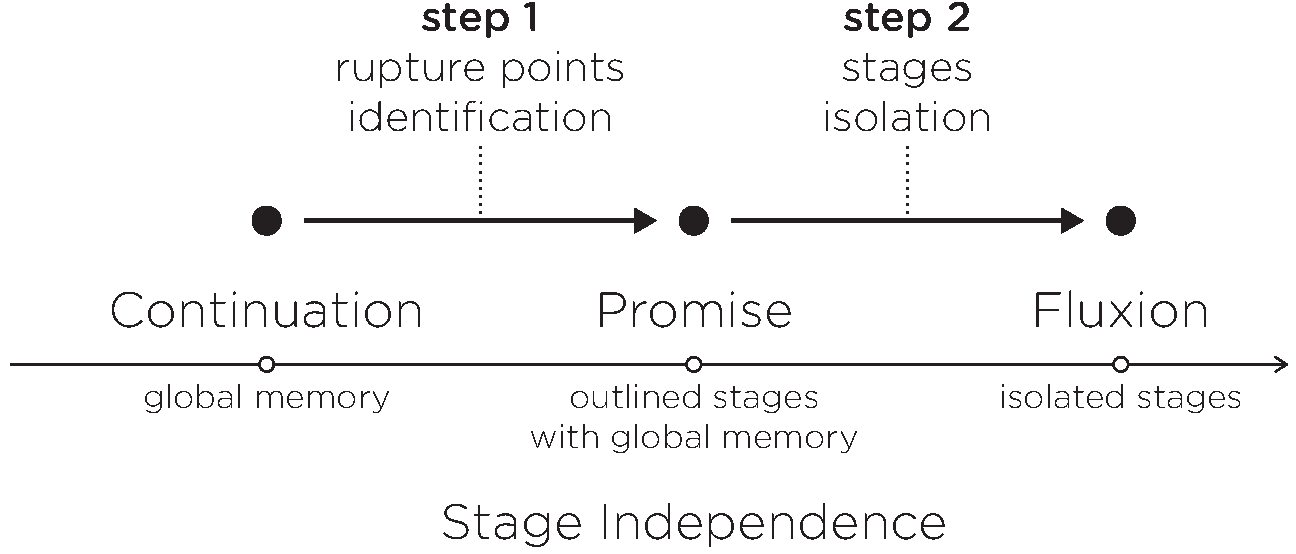
\includegraphics[width=0.9\textwidth]{../resources/roadmap.pdf}
\end{center}
\caption{Roadmap}
\label{fig:roadmap}
\end{figure}

\subsection{Rupture Point}

The pipeline architecture enforces the memory isolation between stages.
Each stage has its own thread of execution, and is independent from the others.
On the other hand, the execution flow of the event-loop jumps from one concurrent task to the other.
%  because of the continuation passing style and the common memory store.
% The message passing linking the callbacks is transparently handled by the event-loop.
However, the executions of these tasks are as distinct as the execution of the different stages of a pipeline.
The call stacks of two concurrent tasks are distinct.
The asynchronous function call between the caller and its continuation represents the rupture between two call stacks.
It is a rupture point, and is equivalent to a data stream between two stages in the pipeline architecture.

Both the pipeline architecture and the event-loop present these rupture points.
The detection of rupture points allows to map a pipeline architecture onto the implementation following the event-loop model.
To allow the transformation from one to the other, this thesis studies the possibility to detect rupture points, and to distribute the global memory into the parts defined by these rupture points.

The detection of rupture points is addressed in chapter \ref{chapter5}.
It presents the extraction of a pipeline of concurent tasks from a Javascript application.
Such pipeline is similar to the one exposed by Promises.
% The chapter proposes a simpler alternative to the latter called Dues.
However, these concurent tasks still require a global memory.
They can't be executed in parallel.

\subsection{Invariance}

% This transformation is important on two points.
% The conservation of the invariance.
% The equivalence between the coordinations.

The global memory assures the total ordering of tasks, and requires sequentiality, while message passing assures causal ordering of tasks and allows parallelism.
The causal ordering of tasks, by opposition to total ordering, is sufficient to assure the correctness of the execution.
Therefore, to assure the correctness of the execution, the ordering allowd by the global memory is partially equivalent to message passing ordering.
And it is possible to transform the global memory coordination into message passing.
% Given that the tasks are independent and communicate by messages.

% This result was used by Lamport to prove the correctness of distributed systems.
Yet, to preserve the correctness as expressed by the developer, it is important to preserve the invariance.
The global memory needs not to be distributed into each of the stages of the pipeline, so that each stage have an exclusive access to its memory.

To assure the missing coordinations assured by the shared memory between the stages, the transformation should provide equivalent coordination with message passing.
The isolation and replacement of the global memory is addressed in chapter \ref{chapter6}, with the introduction of isolated containers called Fluxions.




% The invariance holds for the whole memory during the execution of each callback.
% As I explained in the previous section, this invariance is required to allow the concurrent execution of the different tasks.
% On the other hand, the invariance is explicit in the pipeline architecture, as all the stages have isolated memories.
% The coordination between these isolated process is made explicit by the developer through message passing.

% I argue that the state coordination between the callbacks requireing a global memory could be replaced by the message passing coordination used manually in the pipeline architecture.
% I argue that not all applications need concurrent access on the state, and therefore, need a shared memory.
% % Specifically, I argue that each state region remains roughly local to a stage during its modification.
% \nt{TODO review that, I don't know how to formulate these paragraphs. Identify the state and the data in the global memory.}

% \subsubsection{Transformation}

% This equivalence should allow the transformation of an event loop into several parallel processes communicating by messages.
% In this thesis, I study the static transformation of a program, but the equivalence should also hold for a dynamic transformation.
% I present the analyzis tools I developed to identify the state and the data from the global memory.